\documentclass{article}
\usepackage{amsmath}
\usepackage{amssymb}
\usepackage[usenames, dvipsnames]{color}
\usepackage{fancyhdr}
\usepackage{hyperref}
\usepackage{tikz}
\usepackage{geometry}
\usepackage[normalem]{ulem}

\geometry{letterpaper, portrait, margin=0.5in}
\pagestyle{fancy}

\fancyhf{} % clear all header fields
\renewcommand{\headrulewidth}{0pt}
\fancyfoot[LE,RO]{\thepage}           % page number in "outer" position of footer line
\fancyfoot[RE,LO]{\copyright\;aquarc 2025. \href{https://aquarc.org}{\underline{aquarc.org}}} % other info in "inner" position of footer line

\definecolor{myred1}{RGB}{255, 0, 0}
\definecolor{myyellow1}{RGB}{255, 255, 219}
\definecolor{mygreen1}{RGB}{0, 255, 0}
\definecolor{mygreen2}{RGB}{0, 126, 0}
\definecolor{myblue1}{RGB}{0, 0, 255}

\begin{document}

\fontsize{14}{16}\selectfont

% center the title
\begin{center}
    \textbf{\underline{Sets Cheatsheet}}
\end{center}

\tableofcontents
\pagebreak

\section{Geometric Series}
Geometric Series are a special type of Power Series that can be rewritten in the form

$$
f(x)=\frac{a_1}{1-r}=\sum_{n=0}^{\infty}{
    a_1\cdot r^n
}
$$

\subsection{Proof}
\begin{align*}
    S=a_1+a_1r+a_1r^2+a_1r^3+...+a_1r^n+... \\
    rS=a_1r+a_1r^2+a_1r^3+a_1r^4...+a_1r^n+... \\
    S-rS=a_1+a_1r-a_1r+a_1r^2-a_1r^2+...+a_1r^n-a_1r^n+a_1r^{n+1}+... \\
    \Longrightarrow S(1-r)=a_1+a_1r^{n+1}
\end{align*}
Evaluate the $\lim$ as $n \to \infty$

\begin{align*}
    S=\lim_{n \to \infty}{\frac{a_1+a_1r^{n+1}}{1-r}}
\end{align*}

We can only evaluate this equation when $|r|<1$. Therefore:
$$
\frac{a_1}{1-r}
$$
Is the sum of the geometric series.

To find the interval of convergence, just remember that $|r|< 1$

\subsection{Examples}
$$
f(x)=\frac{1}{2-x}, c=0 
\Longrightarrow f(x)=\frac{1}{2}\cdot \frac{1}{1-\frac{x}{2}}
\Longrightarrow f(x)=\sum_{n=0}^{\infty}{\frac{1}{2}\cdot \biggr(\frac{x}{2}\biggr)^n}
$$
$$
\Longrightarrow f(x)=\sum_{n=0}^{\infty}{\biggr(\frac{1}{2}\biggr)^{n+1}x^n}
$$
$$
|r|<1 
\Longrightarrow \biggr|\frac{x}{2}\biggr|<1
\Longrightarrow |x|<2
\Longrightarrow x \in (-2,2)
$$

If we change the center:
$$
f(x)=\frac{1}{2-x}, c=5 \Longrightarrow f(x)=\frac{1}{2-5-(x-5)} 
\Longrightarrow \frac{1}{-3-(x-5)}
$$
$$
\Longrightarrow -\frac{1}{3}\cdot \frac{1}{1-\frac{-(x-5)}{3}}
\Longrightarrow \sum_{n=0}^{\infty}{-\frac{1}{3}\cdot (\frac{-(x-5)}{3})^n}
$$
$$
\Longrightarrow \sum_{n=0}^{\infty}{(-\frac{1}{3})^{n+1}(-(x-5))^n}
$$
$$
|r|<1
\Longrightarrow r \in (-1,1)
\Longrightarrow \frac{-x+5}{3} \in (-1,1)
\Longrightarrow -(x-5) \in (-3,3)
\Longrightarrow x \in (2,8)
$$
 
Now let's completely change it up.

$$
f(x)=\frac{3}{2x-1}, c=0 
\Longrightarrow f(x)=-3\cdot \frac{1}{1-2x}
\Longrightarrow \cdot \sum_{n=0}^{\infty}{-3\cdot (2x)^n}, c \in (-\frac{1}{2},\frac{1}{2})
$$
Let's move the center
$$
f(x)=\frac{3}{2x-1}, c=-3
\Longrightarrow f(x)=\frac{1}{2(x+3)-5-6}
\Longrightarrow f(x)=-\frac{1}{11}\cdot \frac{1}{1-\frac{2}{11}(x+3)}
$$
$$
f(x)=\sum_{n=0}^{\infty}{-\frac{1}{11}\cdot (\frac{2}{11}(x+3))^n}
$$
$$
\frac{2}{11}(x+3) \in (-1,1) 
\Longrightarrow (x+3) \in (-\frac{11}{2},\frac{11}{2}) 
\Longrightarrow x \in (-\frac{17}{2},\frac{5}{2})
$$

What if there is no $-x$? You can just do $-(-x)$. Remember: Basic Algebra will take you a long way.

$$
f(x)=\frac{3}{x+2}, c=0 \Longrightarrow f(x)=\frac{3}{2}\cdot \frac{1}{1-\frac{1}{2}(-x)}
$$

What if your function looks a bit more complicated?
$$
f(x)=\frac{4x-7}{2x^2+3x-2}, c=0
\Longrightarrow f(x)=\frac{4x-7}{(2x-1)(x+2)}
\Longrightarrow f(x)=\frac{A}{2x-1}+\frac{B}{x+2}
$$
$$
A(x+2)+B(2x-1)=4x-7 
\Longrightarrow Ax+2Bx=4x, 2A-B=-7
\Longrightarrow B=2A+7 
$$
$$
\Longrightarrow A+4A+14=4 
\Longrightarrow 5A=-10 
\Longrightarrow A=-2, B=3
$$
$$
f(x)=\frac{-2}{2x-1}+\frac{3}{x+2}
$$
Solve it normally from here.

\section{General Power Series}
$$
f(x)=\sum_{n=0}^{\infty}{\frac{f^{(n)}(c)}{n!}(x-c)^n}
$$

\subsection{Derivation}
We take general power series to be something like the following:
$$
f(x)=1+x+2x^2+3x^3+...+nx^n+...
$$
or
$$
f(x)=1+x+\frac{1}{2}x^2+\frac{1}{3}x^3+...+\frac{1}{n}x^n+...
$$

So generally:
$$
f(x)=\sum_{n=0}^{\infty}{a_n(x-c)^n}
$$
Instead of $a_i$ because the coefficient changes for each element in the series. Let's expand this series:

$$
f(x)=a_0+c+a_1(x-c)+a_2(x-c)^2+a_3(x-c)^3+...+a_n(x-c)^n + ...
$$
Take its derivative:
$$
f'(x)=0+a_1+2a_2(x-c)+3a_3(x-c)^2+...+na_n(x-c)^{n-1}+...
$$
Notice how $f'(0)=a_1$.
$$
f''(x)=0+0+2a_2+6a_3(x-c)+...+n(n-1)a_n(x-c)^{n-2}+...
$$
Notice how $f''(0)=2a_2$ and $f'''(0)=6a_3$. In order to get the $a_n$ term, you just need to take $f^{(n)}(c)$ and divide it by $n!$ \\
Put it together, and you'll get the equation we started with.

\subsection{Examples}
$$
f(x)=e^x,c=0
\Longrightarrow f(x)=\sum_{n=0}^{\infty}{\frac{e^0}{n!}(x)^n}
\Longrightarrow f(x)=\sum_{n=0}^{\infty}{\frac{x^n}{n!}}
$$
$$
\Longrightarrow 1+x+\frac{1}{2}x^2+\frac{1}{3}x^3+...+\frac{1}{n}x^n+...
$$
Evaluate a geometric series using Taylor series
$$
f(x)=\frac{1}{1-2x},c=0
\Longrightarrow \frac{\frac{1}{1-2(0)}}{0!}+
\frac{\frac{2}{(1-2c)^2}}{1!}x +
\frac{\frac{8}{(1-2c)^3}}{2!}x +
\frac{\frac{48}{(1-2c)^4}}{3!}x+...
$$
$$
\Longrightarrow 1+\frac{2}{(1-2c)^2}x+\frac{4}{(1-2c)^3}x^2+\frac{8}{(1-2c)^4}x^3+...
$$
General term: $2^nx^n$. \\

We would have gotten the same thing if we used the power series expansion of the Taylor series expansion. As with most things in algebra, pick the method that's \textbf{most conveinient for you}.

\subsection{Error Checking}
In an ideal world, you want to know how far off your estimates are. For alternating series, this process is pretty easy.

$$
f(x)=1-x+\frac{x}{2!}-\frac{x}{3!}+\frac{x}{4!}-\frac{x}{5!}+\frac{x}{6!}-\frac{1}{7!}+...+\frac{1}{n!}(-1)^n+...
$$
Let's choose the first four terms for our \textbf{Taylor Polynomial}, which will be represented by $P_n(x)$ where $n$ is the degree.
$$
P_4(x)=1-x+\frac{1}{2}x^2-\frac{1}{3}x^3
$$
Let's set the remainder terms to $R_5(x)$. We can call the error $E(x)$.

$$
E(x)=|P_4(x)-R_5(x)|
$$

Since you will never truly know $R_5(x)$ or any $R_n(x)$ for that matter, you will never know the true error. But you can set an upper bound on that error, which is pretty easy in alternating power series.\\

$$
E(x)\leq P_{n+1}(x) - P_{n}(x)
$$
A fancy way of saying, the term right after is the highest the eror can be. It's because you will never add back what you subtracted, always less.

\subsection{Deriving $e^a$}
We can use a Taylor Series to derive $e^a$!
\begin{align*}
    \lim_{n \to \infty}{(1+\frac{a}{n})^n}=L
    \Longrightarrow \ln(\lim_{n \to \infty}{(1+\frac{a}{n})^n})=\ln L
    \Longrightarrow n\ln(\lim_{n \to \infty}{(1+\frac{a}{n})})=\ln L \\
    t=\frac{a}{n}, \Longrightarrow \frac{a}{t}(\lim_{n \to \infty}{\ln(1+t)})=\ln L
    \Longrightarrow \frac{a}{t}(\lim_{t \to 0}{\ln(1+t)})=\ln L \\
    \longrightarrow \ln(1+t)=t-\frac{t^2}{2}+\frac{t^3}{3}+...\approx t \\
    \Longrightarrow \ln L=a \Longrightarrow L=e^a
\end{align*}

\subsection{Lagrange Error Checking}
If your series \textbf{isn't alternating}, you can use Lagrange Error Checking. Although the proof is complicated, it's pretty simple
$$
E(x)\leq|\frac{\max_{z \in [x,c]}{f^{(n+1)}(z)}}{(n+1)!}|(x-c)^{n+1}
$$

The proof isn't necessary for Calc BC. You can find it online. 
\subsubsection{Full Example}
Find the first four terms about $c=2$ for $ln|x+1|$. 

We can start with its derivative, $\frac{1}{x+1}$.\\
For simplicity, we will use a geometric series.
Say we wanted to find $\ln|\frac{3}{2}|$ and approximate error to be 0.05 or less

\begin{align*}
    \frac{1}{x-1}=\frac{1}{1-(x-2)+2}=\frac{1}{-1-(x-2)}=-\frac{1}{1-(-(x-2))} \\
    \Longrightarrow \sum_{n=0}^{\infty}{-(-(x-2))^n} = 
    \sum_{n=0}^{\infty}{(-1)^{n+1}(x-2)^n} = -1+(x-2)-\frac{1}{2}(x-2)^2+\frac{1}{3}(x-2)^3+... \\
    \int{-\frac{1}{1-(-(x-2))}}dx = \int{-1+(x-2)-\frac{1}{2}(x-2)^2+\frac{1}{3!}(x-2)^3+...}dx \\
    \Longrightarrow -\ln|1-(-(x-2))|=C-x+\frac{(x-2)^2}{2}-\frac{(x-2)^3}{3\cdot 2!}+\frac{(x-2)^4}{4\cdot 3!}+... \\
    \longrightarrow \ln|1-(-(2-2))|=\ln|1| \\
    \longrightarrow C+x-\frac{(x-2)^2}{2}+\frac{(x-2)^3}{3\cdot 2!}-\frac{(x-2)^4}{4\cdot 3!}+... \\
    \longrightarrow \ln|1|=C+2+0+... \longrightarrow C=-2 \\
    \Longrightarrow \ln|1-(-(x-2))|=-2+x-\frac{(x-2)^2}{2}+\frac{(x-2)^3}{3\cdot 2!}-\frac{(x-2)^4}{4\cdot 3!}+... \\
    \Longrightarrow \ln|\frac{3}{2}|=\ln|1-(-(\frac{5}{2}-2))|=
    (\frac{5}{2}-2)-\frac{(\frac{5}{2}-2)^2}{2}
    +\frac{(\frac{5}{2}-2)^3}{3\cdot 2!}-\frac{(\frac{5}{2}-2)^4}{4\cdot 3!}+...\\
    \Longrightarrow  \frac{1}{2}-\frac{1}{2}\cdot (\frac{1}{2})^2+\frac{1}{3}\cdot (\frac{1}{2})^3
    -\frac{1}{4}\cdot (\frac{1}{2})^4+...\\
\end{align*}
Since it's an alternating series, it should be pretty simple to solve for from here.
\subsubsection{Another Problem}
$$
\sin(5x+\frac{\pi}{4})=\sin(5(x+\frac{\pi}{20}))
$$
% yeah i'm not doing this lol

\section{P Series}
\textbf{NOT} Power Series. \\ 

A P Series is any series in the form:
$$
\sum_{n=0}^{\infty}{\frac{1}{n^p}}
$$
We use Integral Test to prove if it is diverging or converging.

\subsection{Harmonic Series}

A Harmonic Series is:
$$
\sum_{n=0}^{\infty}{\frac{1}{n}}
$$

Or a P Series where $p=1$.

\subsection{Proof}
Where $p=1$ (Harmonic Series)

\begin{align*}
    \int_{1}^{\infty}{\frac{1}{x}}dx < \sum_{n=1}^{\infty}{\frac{1}{n}} < \int_{1}^{\infty}{\frac{1}{x}}dx + 1
    \Longrightarrow \int_{1}^{\infty}{\frac{1}{x}}dx = \ln|x|\biggr\rvert^{\infty}_{1} \\
    \Longrightarrow \lim_{x \to \infty}{\ln x} = \infty
\end{align*}
Diverges\\

Where $p\neq 1$

\begin{align*}
    \int_{1}^{\infty}{\frac{1}{x^p}}dx < \sum_{n=1}^{\infty}{\frac{1}{n^p}} < \int_{1}^{\infty}{\frac{1}{x^p}}dx + 1
    \longrightarrow \int_{1}^{\infty}{x^{-p}}dx = \frac{x^{-p+1}}{-p+1}\biggr\rvert^{\infty}_{1} \\
    \longrightarrow \lim_{x \to \infty}{\frac{x^{-p+1}}{-p+1}}
\end{align*}
If $p>1$ it converges, $p<1$ (or $p\leq 1$) it diverges.

\subsection{Examples}

\begin{align*}
    \sum_{n=1}^{\infty}{\frac{1}{(2n+3)^2}}
    \Longrightarrow \int_1^{\infty}{\frac{1}{(2x+3)^2}}dx 
    \longrightarrow u=2x+3 \quad du=2dx
    \Longrightarrow \int_3^{\infty}{\frac{1}{2u^3}}du
\end{align*}
Convergent

\begin{align*}
    \sum_{n=1}^{\infty}{\frac{n+2}{n+1}}
    \Longrightarrow \int_1^{\infty}{\frac{x+2}{x+1}}dx=\int_1^{\infty}{(1+\frac{1}{x+1})}dx
    = (x+ \ln |x+1|)\biggr\rvert^{\infty}_{1}\\
    = \lim_{x \to \infty}{x+ \ln |x+1|} = \infty
\end{align*}
Divergent

\section{Convergent or Divergent}

\subsection{nth Term Test for Divergence}
If
$$
\lim_{x \to \infty}a_x\neq 0
$$
then $f$ is divergent. If
$$
\lim_{x \to \infty}a_x=0
$$
then use another test, it's inconclusive.

\subsection{Ratio Test}

Commonly used for geometric series, if you just check to make sure $|r|<1$ then it's going to converge. 

$$
\lim_{n \to \infty}{|\frac{a^{n+1}}{a^n}|}
$$

Basically checking that for some far off value, the common ratio remains. \\
Example:

\begin{align*}
    \sum_{n=0}^{\infty}{\frac{(-1)^{n-1}n^2}{2^n}}
    \Longrightarrow \lim_{n \to \infty}{|\frac{\frac{(-1)^{n}(n+1)^2}{2^{n+1}}}
        {\frac{(-1)^{n-1}n^2}{2^n}}|}=0
    \Longrightarrow \lim_{n \to \infty}{|\frac{(-1)^{n}(n+1)^2\cdot 2^n}{2^n\cdot 2\cdot (-1)^{n-1}n^2}|} \\
    \Longrightarrow \lim_{n \to \infty}{|\frac{(n+1)^2}{2\cdot -1\cdot n^2}|}=\frac{1}{2}
\end{align*}

If $|r|=1$, we have a problem. Recall the limit from the geometric series proof:
$$
\lim_{n \to \infty}{\frac{a-ar^{n+1}}{1-r}}
$$

That's going to be undefined. So we have to use another test.

This test is best used for rapidly growing questions like $n!$.

\subsubsection{More Examples}

\begin{align*}
    \sum_{n=0}^{\infty}{\frac{e^n}{n^3}} \Longrightarrow \lim_{n \to \infty}{|\frac{\frac{e^n\cdot e}{(n+1)^3}}{\frac{e^n}{n^3}}|}
    \Longrightarrow \lim_{n \to \infty}{|\frac{e\cdot n^3}{(n+1)^3}|}=e\not < 1
\end{align*}
Divergent
\begin{align*}
    \sum_{n=0}^{\infty}{\frac{(n!)^2}{(3n)!}}
    \Longrightarrow \lim_{n \to \infty}{|\frac{\frac{((n+1)!)^2}{(3n+3)!}}{\frac{(n!)^2}{(3n)!}}|}
    \Longrightarrow \lim_{n \to \infty}{|\frac{((n+1)!)^2\cdot (3n)!}{(3n+3)!\cdot (n!)^2}|} \\
    \Longrightarrow \lim_{n \to \infty}{|\frac{(n+1)^2\cdot (n!)^2\cdot (3n)!}{(3n+3)\cdot (3n+2)\cdot (3n+1)\cdot (3n)!\cdot (n!)^2}|} \\
    \Longrightarrow \lim_{n \to \infty}{|\frac{(n+1)^2}{(3n+3)\cdot (3n+2)\cdot (3n+1)}|}=0<1
\end{align*}
Convergent
\begin{align*}
    \sum_{n=0}^{\infty}{\frac{n!}{n^{n+1}}}
    \Longrightarrow \lim_{n \to \infty}{|\frac{\frac{(n+1)!}{(n+1)^{n+2}}}{\frac{n!}{n^{n+1}}}|}
    \Longrightarrow \lim_{n \to \infty}{|\frac{(n+1)!\cdot n^{n+1}}{n!\cdot (n+1)^{n+2}}|}
    \Longrightarrow \lim_{n \to \infty}{|\frac{n!\cdot n^{n+1}}{n!\cdot (n+1)^{n+1}}|} \\
    \Longrightarrow \lim_{n \to \infty}{|(\frac{n}{n+1})^{n+1}|}=
                    \lim_{n \to \infty}{|(\frac{n+1-1}{n+1})^{n+1}|}=
                    \lim_{n \to \infty}{|(1-\frac{1}{n+1})^{n+1}|}=\\
                    \lim_{n \to \infty}{|(1+\frac{(-1)}{n+1})^{n+1}|}=e^{-1}<1
\end{align*}
Convergent
\begin{align*}
    \sum_{n=1}^{\infty}{\frac{3^{1-2n}}{n^2+1}}
    \Longrightarrow \lim_{n \to \infty}{|\frac{\frac{3^{1-2n-2}}{(n+1)^2+1}}{\frac{3^{1-2n}}{n^2+1}}|}
    \Longrightarrow \lim_{n \to \infty}{|\frac{3^{-1-2n}\cdot (n^2+1)}{(n+1)^2+1\cdot 3^{1-2n}}|} \\
    \Longrightarrow \lim_{n \to \infty}{|\frac{n^2+1}{(n+1)^2+1\cdot 3^{1-2n}\cdot 3^{1+2n}}|}
    \Longrightarrow \lim_{n \to \infty}{|\frac{n^2+1}{(n+1)^2+1\cdot 3\cdot 3^{-2n}\cdot 3\cdot 3^{2n}}|} \\
    \Longrightarrow \lim_{n \to \infty}{|\frac{n^2+1}{(n+1)^2+1\cdot 3\cdot 3}|}=\frac{1}{9}
\end{align*}
Convergent
\begin{align*}
    \sum_{n=2}^{\infty}{\frac{(-2)^{1+3n}(n+1)}{n^25^{1+n}}} \\
    \Longrightarrow \lim_{n \to \infty}{|\frac{\frac{(-2)^{4+3n}(n+2)}{(n+1)^25^{2+n}}}{\frac{(-2)^{1+3n}(n+1)}{n^25^{1+n}}}|}
    \Longrightarrow \lim_{n \to \infty}{|\frac{(-2)^{4+3n}(n+2)n^25^{1+n}}{(n+1)^25^{2+n}(-2)^{1+3n}(n+1)}|} \\
    \Longrightarrow \lim_{n \to \infty}{|\frac{(-2)^{3}(n+2)n^2}{(n+1)^35}|}=\frac{(-2)^3}{5^5}=-\frac{8}{5}
\end{align*}
Diverges

\begin{align*}
    \sum_{n=1}^{\infty}{\frac{(-1)^{n+1}}{6n+7}}
    \Longrightarrow \lim_{n \to \infty}{|\frac{\frac{(-1)^{n+2}}{6n+6+7}}{\frac{(-1)^{n+1}}{6n+7}}|}
    \Longrightarrow \lim_{n \to \infty}{|\frac{(-1)^{n+2}(6n+7)}{(6n+6+7)(-1)^{n+1}}|} \\
    \Longrightarrow \lim_{n \to \infty}{|\frac{6n+7}{6n+6+7}|}
\end{align*}
Inconclusive: But if you used the Divergence Test first:
\begin{align*}
    \lim_{n \to \infty}{\frac{(-1)^{n+1}}{6n+7}}\approx \frac{(-1)^{\infty}}{\infty}=0
\end{align*}
Inconclusive, but the alternating series test proves it right.

\begin{align*}
    \sum_{n=3}^{\infty}{\frac{e^{4n}}{(n-2)!}} \\
    \longrightarrow \lim_{n \to \infty}{\frac{e^{4n}}{(n-2)!}} = 0 \\
    \Longrightarrow \lim_{n \to \infty}{|\frac{\frac{e^{4n+4}}{(n-1)!}}{\frac{e^{4n}}{(n-2)!}}|} 
    \Longrightarrow \lim_{n \to \infty}{|\frac{e^{4n+4}(n-2)!}{(n-1)!e^{4n}}|} 
    \Longrightarrow \lim_{n \to \infty}{|\frac{e^4(n-2)!}{(n-1)(n-2)!}|} 
    \Longrightarrow \lim_{n \to \infty}{|\frac{e^4}{(n-1)}|} \\
    \Longrightarrow 0
\end{align*}
Convergent

\subsection{Integral Test}
If $f(x)$ is decreasing, then for $x\geq 1$:

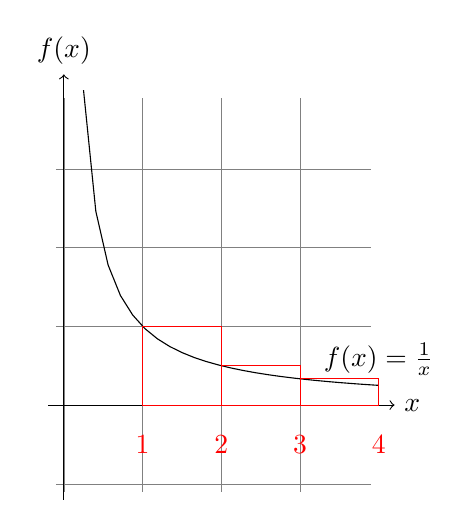
\begin{tikzpicture}[domain=0.25:4]
    \draw[very thin,color=gray] (-0.1,-1.1) grid (3.9,3.9);
    \draw[->] (-0.2,0) -- (4.2,0) node[right] {$x$};
    \draw[->] (0,-1.2) -- (0,4.2) node[above] {$f(x)$};
    \draw plot (\x,1/\x) node[above] {$f(x) =\frac{1}{x}$};
    \draw[color=red] (1,0) rectangle (2,1);
    \draw[color=red] (2,0) rectangle (3,0.5);
    \draw[color=red] (3,0) rectangle (4,0.333);
    \draw[color=red] (1,-0.5) node {$1$};
    \draw[color=red] (2,-0.5) node {$2$};
    \draw[color=red] (3,-0.5) node {$3$};
    \draw[color=red] (4,-0.5) node {$4$};
\end{tikzpicture}
The Left Riemann Sum is $>$ than $f(x)$:
\begin{align*}
    \frac{1}{1}+\frac{1}{2}+\frac{1}{3}+... 
    \Longrightarrow \sum_{n=1}^{\infty}{\frac{1}{n}} > \int_{1}^{\infty}{\frac{1}{x}}dx
\end{align*}
Similarly, \\
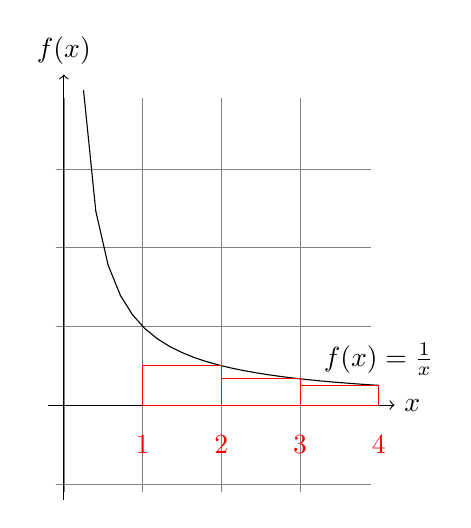
\begin{tikzpicture}[domain=0.25:4]
    \draw[very thin,color=gray] (-0.1,-1.1) grid (3.9,3.9);
    \draw[->] (-0.2,0) -- (4.2,0) node[right] {$x$};
    \draw[->] (0,-1.2) -- (0,4.2) node[above] {$f(x)$};
    \draw plot (\x,1/\x) node[above] {$f(x) =\frac{1}{x}$};
    \draw[color=red] (1,0) rectangle (2,0.5);
    \draw[color=red] (2,0) rectangle (3,0.3333);
    \draw[color=red] (3,0) rectangle (4,0.25);
    \draw[color=red] (1,-0.5) node {$1$};
    \draw[color=red] (2,-0.5) node {$2$};
    \draw[color=red] (3,-0.5) node {$3$};
    \draw[color=red] (4,-0.5) node {$4$};
\end{tikzpicture}
The Right Riemann Sum is $<$ than $f(x)$:
\begin{align*}
    \frac{1}{2}+\frac{1}{3}+\frac{1}{4}+... 
    \Longrightarrow \sum_{n=2}^{\infty}{\frac{1}{n}} < \int_{1}^{\infty}{\frac{1}{x}}dx \\
    \Longrightarrow \sum_{n=\textcolor{myred1}{1}}^{\infty}{\frac{1}{n}} < \int_{1}^{\infty}{\frac{1}{x}}dx + 1 \\
    \Longrightarrow \int_{1}^{\infty}{\frac{1}{x}}dx < \sum_{n=1}^{\infty}{\frac{1}{n}} < \int_{1}^{\infty}{\frac{1}{x}}dx + 1
\end{align*}

Using a method analogous to the Squeeze Theorem, if the bounds diverge, so does the series, and vice versa.

\subsection{Direct Comparison Test}

The direct comparison test allows for \textbf{no negative terms} in the series.\\

Let $a_n$ and $b_n$ represent an unknown and known sequence, respectively. \\

If $a_n < b_n$ for all $n$ (according to CollegeBoard, however the first few terms are an exception) and $\lim_{n \to \infty}{\sum_i^n{b_i}}=L$
then $\lim_{n \to \infty}{\sum_i^n{a_i}=L_2}$ \\

If $a_n > b_n$ for all $n$ and $\lim_{n \to \infty}{\sum_i^n{b_i}}=L$
then $\lim_{n \to \infty}{\sum_i^n{a_i}}$ could equal $L_2$ or $\infty$. \\

If $a_n < b_n$ for all $n$ and $\lim_{n \to \infty}{\sum_i^n{b_i}}=\infty$
then $\lim_{n \to \infty}{\sum_i^n{a_i}}$ could equal $L_2$ or $\infty$.\\

If $a_n > b_n$ for all $n$ and $\lim_{n \to \infty}{\sum_i^n{b_i}}=\infty$
then $\lim_{n \to \infty}{\sum_i^n{a_i}}=\infty$. \\

It is recommended to use this test only if the degree is the same.

\subsubsection{Examples}

\begin{align*}
    \sum_{n=2}^{\infty}{\frac{1}{n^2+1}}=\frac{1}{5}+\frac{1}{10}+\frac{1}{17}+...\\
    \sum_{n=2}^{\infty}{\frac{1}{n^2}}=\frac{1}{4}+\frac{1}{9}+\frac{1}{16}+...\\
    \Longrightarrow \sum_{n=2}^{\infty}{\frac{1}{n^2}} > \sum_{n=2}^{\infty}{\frac{1}{n^2+1}} 
    \Longrightarrow \sum_{n=2}^{\infty}{\frac{1}{n^2}} = L \therefore \sum_{n=2}^{\infty}{\frac{1}{n^2+1}} = L_2
\end{align*}
Convergent

\subsection{Limit Comparison Test}
$$
\lim_{n \to \infty}{\frac{a_n}{b_n}}
$$
For $0<n<\infty$ (if it is 0 or $\infty$ anyway, the previous test would suffice).

\subsubsection{Examples}
\begin{align*}
    \sum_{n=1}^{\infty}{\frac{n}{n^2+1}}=\frac{1}{2}+\frac{2}{5}+\frac{3}{10}+...\\
    \sum_{n=1}^{\infty}{\frac{n}{n^2}}=\frac{1}{1}+\frac{1}{2}+\frac{1}{3}+...\\
    \Longrightarrow \sum_{n=1}^{\infty}{\frac{1}{n}} > \sum_{n=1}^{\infty}{\frac{n}{n^2+1}} 
    =\lim_{n \to \infty}{\frac{1}{n}} > \lim_{n \to \infty}{\frac{n}{n^2+1}}
    =\infty > \lim_{n \to \infty}{\frac{n}{n^2}}
\end{align*} 
Inconclusive
\begin{align*}
    \lim_{n \to \infty}{\frac{\frac{n}{n^2+1}}{\frac{1}{n}}}
    =\lim_{n \to \infty}{\frac{n^2}{n^2+1}}=1
\end{align*}
Convergent
\begin{align*}
    \sum_{n=1}^{\infty}{\frac{5n-3}{n^2-2n+5}}=\frac{-3}{5}+\frac{2}{4}+\frac{7}{5}+
        \frac{12}{8}+\frac{17}{13}...\\
    \sum_{n=1}^{\infty}{\frac{n}{n^2}}=\frac{1}{1}+\frac{1}{2}+\frac{1}{3}+
        \frac{1}{4}+\frac{1}{5}...\\
    \Longrightarrow \lim_{n \to \infty}{\frac{\frac{5n-3}{n^2-2n+5}}{\frac{1}{n}}} =
        \lim_{n \to \infty}{\frac{5n^2-3n}{n^2-2n+5}}=5 \\
    \lim_{n \to \infty}{\frac{1}{n}}=\infty \therefore \lim_{n \to \infty}{\frac{5n-3}{n^2-2n+5}}=\infty
\end{align*}
Divergent

\subsection{Alternating Series \sout{Property} Theorem}

Recall the Alternating Error Bound for a series. Take this example:

\begin{align*}
    \sum_{n=1}^{\infty}{\frac{(-1)^{n+1}}{n}}=\frac{1}{1}-\frac{1}{2}+\frac{1}{3}-\frac{1}{4}+...
\end{align*}

Since the sum is \textbf{decreasing} and $\lim_{n \to \infty}{\frac{1}{n}}=0$ (since $n$ is increasing), there is an error bound, meaning this alternating series is convergent. Note that this "test" doesn't apply to oscillating serieses like $sin(x)$. \\

\subsubsection{Example}

\begin{align*}
    \sum_{n=1}^{\infty}{\frac{(-1)^{n+1}n}{2n+1}}\\
    \lim_{n \to \infty}{\frac{n}{2n+1}}=\frac{1}{2} 
    \Longrightarrow \approx \sum_{n=1}^{\infty}{\frac{(-1)^{n+1}}{2}}
\end{align*}
This sum does not reach 0, it osciilates. It is not convergent.

\subsection{Absolute Convergence Test}
Let $a_n$ represent a sequence with positive and negative terms. \\

Using some common sense, we can derive the following:

\begin{align*}
    n \in \mathbb{R} \Longrightarrow n \leq |n| \\
    \therefore a_n \leq |a_n| \\
    \Longrightarrow a_n + |a_n| \leq 2 |a_n| \\
    \longrightarrow |a_n| + a_n = 0 \quad\text{or}\quad 
    2a_n \therefore 0 \leq a_n+|a_n| \leq 2a_n
\end{align*}

By the Direct Comparsion test:
\begin{align*}
    \sum_{n=1}^{\infty}{|a_n|} = L \therefore \sum_{n=1}^{\infty}{a_n} = L_2
\end{align*}
In this case it is absolutely convergent. In the scenario that:
\begin{align*}
\sum_{n=1}^{\infty}{|a_n|} = \infty
\end{align*}
It is inconclusive. If the other alternating series tests passes, it is \textbf{Conditionally Convergent}.

\subsection{Examples}

\begin{align*}
    \sum_{n=2}^{\infty}{\frac{n}{\ln n}}
    \Longrightarrow \lim_{n \to \infty}{\frac{n}{\ln n}}=\infty
\end{align*}
Divergent by nth Term Test for Divergence

\begin{align*}
    \sum_{n=1}^{\infty}{\frac{2^n}{n^{99}}}
    \Longrightarrow \lim_{n \to \infty}{\frac{2^n}{n^{99}}}=\infty
\end{align*}
Divergent by nth Term Test for Divergence

\begin{align*}
    \sum_{n=1}^{\infty}{\frac{\sqrt{n^2+1}}{n}}
    \Longrightarrow \lim_{n \to \infty}{\frac{\sqrt{n^2+1}}{n}} 
    \approx \lim_{n \to \infty}{\frac{\sqrt{n^2}}{n}}
    =\lim_{n \to \infty}{\frac{n}{n}}=1
\end{align*}
Divergent by nth Term Test for Divergence

\begin{align*}
    \sum_{n=2}^{\infty}{\frac{n^e}{n^{\pi}}}
    =\sum_{n=2}^{\infty}{\frac{1}{n^{\pi-e}}}
    \Longrightarrow 1\geq \pi-e
\end{align*}
Divergent by property of P-Series

\begin{align*}
    \sum_{n=0}^{\infty}{\frac{1}{\sqrt{n+8}}}=\frac{1}{\sqrt{8}}+\sum_{n=1}^{\infty}{\frac{1}{\sqrt{n+8}}}=\frac{1}{\sqrt{8}}+\frac{1}{3}+\frac{1}{\sqrt{10}}+... \\
    \sum_{n=1}^{\infty}{\frac{1}{\sqrt{n}}}=\frac{1}{\sqrt{1}}+\frac{1}{\sqrt{2}}+\frac{1}{\sqrt{3}}+... \\
    \Longrightarrow \lim_{n \to \infty}{\frac{\frac{1}{\sqrt{n+8}}}{\frac{1}{\sqrt{n}}}}
    =               \lim_{n \to \infty}{\frac{\sqrt{n+8}}{\sqrt{n}}}=1
\end{align*}
Divergent by Limit Comparison Test

\begin{align*}
    \sum_{n=1}^{\infty}{\frac{(-1)^n}{n!}}=\frac{1}{1}-\frac{1}{1!}+\frac{1}{2!}-\frac{1}{3!}+...
\end{align*}
Convergent by Properties of Alternating Series:
\begin{enumerate}
    \item It is decreasing
    \item It is approaching 0
    \item It is alternating
\end{enumerate}

\begin{align*}
    \sum_{n=3}^{\infty}{\frac{4}{n\sqrt{\ln n}}}=\frac{4}{3\sqrt{\ln 3}}+\frac{4}{4\sqrt{\ln 4}}+\frac{4}{5\sqrt{\ln 5}}+... \\
    \sum_{n=3}^{\infty}{\frac{4}{n}}=\frac{4}{3}+\frac{4}{4}+\frac{4}{5}+... \\
    \Longrightarrow \sum_{n=3}^{\infty}{\frac{4}{n\sqrt{\ln n}}} < \sum_{n=3}^{\infty}{\frac{4}{n}}, \sum_{n=3}^{\infty}{\frac{4}{n}}=\infty \\
    \Longrightarrow \lim_{n \to \infty}{\frac{\frac{4}{n\sqrt{\ln n}}}{\frac{4}{n}}}=0 \\
    \lim_{n \to \infty}{\frac{\frac{4}{n\sqrt{\ln (n+1)}+\sqrt{\ln (n+1)}}}{\frac{4}{n\sqrt{\ln n}}}}=???
\end{align*}
After trying three tests, we are left with the Integral Test

\begin{align*}
    \sum_{n=3}^{\infty}{\frac{4}{n\sqrt{\ln n}}}  \\
    \Longrightarrow 4\int_3^{\infty}{\frac{1}{n\sqrt{\ln n}}}dn, 
    u=\ln n, \quad du=\frac{1}{n}dn \\
    \Longrightarrow 4\int_{\ln 3}^{\infty}{\frac{1}{\sqrt{u}}}du
    =\int_{\ln 3}^{\infty}{u^{-\frac{1}{2}}}du=4*[2u^{\frac{1}{2}}]\biggr\rvert^{\infty}_{\ln 3}
\end{align*}
Divergent by Integral Test

\begin{align*}
    \sum_{n=1}^{\infty}{\frac{1}{\sqrt[3]{27n^2}}}
    = \frac{1}{3}\sum_{n=1}^{\infty}{\frac{1}{n^{\frac{2}{3}}}}
\end{align*}
Divergent by Property of P-Series

\begin{align*}
    \sum_{n=1}^{\infty}{\frac{n}{\sqrt{n^2+1}}}
    \Longrightarrow \lim_{x \ to \infty}{\frac{x}{\sqrt{x^2+1}}}
    \approx \lim_{x \ to \infty}{\frac{x}{x}}=1
\end{align*}
Divergent by nth Term Test for Divergence

\begin{align*}
    \sum_{n=1}^{\infty}{\sqrt{\frac{n+1}{n}}}
\end{align*}
Be careful, this is NOT a disguised $\frac{1}{e}$. 
\begin{align*}
    \approx \sum_{n=1}^{\infty}{\sqrt{\frac{n}{n}}}=1
\end{align*}

Divergent by nth Term Test for Divergence

\begin{align*}
    \sum_{n=1}^{\infty}{\frac{2^n+3^n}{4^n}}
    =\sum_{n=1}^{\infty}{\frac{2^n}{4^n}+\frac{3^n}{4^n}}
    =\sum_{n=1}^{\infty}{\frac{2^n}{4^n}}+\sum_{n=1}^{\infty}{\frac{3^n}{4^n}}
    =\sum_{n=1}^{\infty}{\biggr(\frac{2}{4}\biggr)^n}
        +\sum_{n=1}^{\infty}{\biggr(\frac{3}{4}\biggr)^n}
\end{align*}

Convergent by Property of Geometric Series

\begin{align*}
    \sum_{n=3}^{\infty}{\frac{1}{n(\ln n)(\ln (\ln n))}}
    =\sum_{n=3}^{\infty}{\frac{1}{n(\ln n)}\frac{1}{(\ln (\ln n))}} \\
    \Longrightarrow \sum_{n=3}^{\infty}{\frac{1}{\ln (\ln n)}} 
    =\frac{1}{\ln (\ln 3)}+\frac{1}{\ln (\ln 4)} + \frac{1}{\ln (\ln 5)} + ... \\
    \sum_{n=3}^{\infty}{\frac{1}{n}}=\frac{1}{3}+\frac{1}{4}+\frac{1}{5}+... \\
    \Longrightarrow \sum_{n=3}^{\infty}{\frac{1}{n}}<\sum_{n=3}^{\infty}{\frac{1}{\ln (\ln n)}} \\
    \sum_{n=3}^{\infty}{\frac{1}{n}}=\infty \therefore \sum_{n=3}^{\infty}{\frac{1}{\ln (\ln n)}}=\infty
\end{align*}

A divergent sum times any sum is divergent. \\
Divergent by Property of P-Series

\begin{align*}
    \sum_{n=3}^{\infty}{\frac{1}{2^n-n}}=\frac{1}{5}+\frac{1}{12}+\frac{1}{27}+...\\
    \sum_{n=3}^{\infty}{\frac{1}{2^n}}=\frac{1}{8}+\frac{1}{16}+\frac{1}{32}+...\\
    \sum_{n=3}^{\infty}{\frac{1}{2^n-n}}>\sum_{n=3}^{\infty}{\frac{1}{2^n}} \\
    \sum_{n=3}^{\infty}{\frac{1}{2^n}}=L\\
    \lim_{n \to \infty}{\frac{\frac{1}{2^n-n}}{\frac{1}{2^n}}}
    =\lim_{n \to \infty}{\frac{2^n}{2^n-n}}=1
\end{align*}
Convergent by Limit Comparison Test

\begin{align*}
    \sum_{n=1}^{\infty}{\frac{5+8^n}{2-7^n}}
    =\sum_{n=1}^{\infty}{\biggr(\frac{5}{2-7^n}+\frac{8^n}{2-7^n}\biggr)}
    =\sum_{n=1}^{\infty}{\biggr(\frac{5}{2-7^n}-\frac{8^n}{7^n-2}\biggr)} \\
    \Longrightarrow \sum_{n=1}^{\infty}{\frac{8^n}{7^n-2}}=\frac{8}{5}+\frac{64}{47}+... \\
    \lim_{n \to \infty}{\frac{8^n}{7^n-2}} 
    \approx \lim_{n \to \infty}{\frac{8^n}{7^n}}
    = \lim_{n \to \infty}{\biggr(\frac{8}{7}\biggr)^n} = \infty
\end{align*}
A divergent series plus any series is divergent. \\
Divergent by nth Term Test for Divergence

\section{More Examples}

\begin{enumerate}

\item \begin{align*}
    \sum_{n=1}^{\infty}{(-1)^n\frac{(x-2)^n}{n+1}}
\end{align*}

For P-Series, you can \textbf{only use} the Ratio Test to determine Convergence over an Interval

\begin{align*}
    \Longrightarrow \lim_{n \to \infty}{\frac{\frac{(-1)^{n+1}(x-2)^{n+1}}{n+2}}{\frac{(-1)^n(x-2)^n}{n+1}}}
    = \lim_{n \to \infty}{\biggr|\frac{(n+1)(-1)^{n+1}(x-2)^{n+1}}{(n+2)(-1)^n(x-2)^n}\biggr|}
    = \lim_{n \to \infty}{\biggr|\frac{(n+1)(x-2)}{(n+2)}\biggr|} \\
    = \lim_{n \to \infty}{|x-2|} < 1 \\
    \Longrightarrow 1 < x < 3 
\end{align*}
Now you have to test the values 1 and 3.

\begin{align*}
    \sum_{n=0}^{\infty}{\biggr|(-1)^n\frac{(x-2)^n}{n+1}\biggr|} \\
    \longrightarrow \sum_{n=0}^{\infty}{\biggr|(-1)^n\frac{(1-2)^n}{n+1}\biggr|} \\
    \longrightarrow \sum_{n=0}^{\infty}{\biggr|(-1)^n\frac{(-1)^n}{n+1}\biggr|} 
    =               \sum_{n=0}^{\infty}{\biggr|\frac{1}{n+1}\biggr|} 
\end{align*}
Divergent by Comparsion Test
\begin{align*}
    \sum_{n=0}^{\infty}{\biggr|(-1)^n\frac{(3-2)^n}{n+1}\biggr|} \\
    \longrightarrow \sum_{n=0}^{\infty}{\biggr|(-1)^n\frac{(1)^n}{n+1}\biggr|} \\
    \longrightarrow \sum_{n=0}^{\infty}{\biggr|\frac{(-1)^n}{n+1}\biggr|} 
    =               \sum_{n=0}^{\infty}{\biggr|\frac{(-1)^n}{n+1}\biggr|} 
\end{align*}
Convergent by Alternating Series "Test"
$$
1 < x \leq 3
$$

\item \begin{align*}
    \sum_{n=1}^{\infty}{\frac{x^nn^n}{3^nn!}} \\
    \Longrightarrow \lim_{n \to \infty}{\biggr|\frac{\frac{x^{n+1}(n+1)^{n+1}}{3^{n+1}(n+1)!}}{\frac{x^nn^n}{3^nn!}}\biggr|}
    = \lim_{n \to \infty}{\biggr|\frac{x^{n+1}(n+1)^{n+1}3^nn!}{x^nn^n3^{n+1}(n+1)!}\biggr|}
    = \lim_{n \to \infty}{\biggr|\frac{x^{n+1}(n+1)(n+1)^{n}n!}{x^nn^n3(n+1)!}\biggr|} \\
    = \lim_{n \to \infty}{\biggr|\frac{x(n+1)^{n}n!}{n^n3n!}\biggr|}
    = \frac{1}{3}\lim_{n \to \infty}{\biggr|x\biggr(\frac{n+1}{n}\biggr)^n\biggr|}
    = \frac{1}{3}\lim_{n \to \infty}{\biggr|x\biggr(1+\frac{1}{n}\biggr)^n\biggr|} \\
    \Longrightarrow \biggr|\frac{e}{3}x\biggr|<1 \Longrightarrow -\frac{3}{e}<x<\frac{3}{e}
\end{align*}
Plug in the endpoints:
\begin{align*}
    \sum_{n=1}^{\infty}{\frac{(-\frac{3}{e})^nn^n}{3^nn!}}
    = \sum_{n=1}^{\infty}{\frac{(-1)^n(3)^nn^n}{e^n3^nn!}}
    = \sum_{n=1}^{\infty}{\frac{(-1)^nn^n}{e^nn!}}
\end{align*}
Look at the graph and compare it against $\frac{1}{n}$.

\item \begin{align*}
    \sum_{k=0}^{\infty}{\frac{2^kx^k}{\ln(k+2)}} \\
    \lim_{k \to \infty}{\biggr|\frac{\frac{2^{k+1}x^{k+1}}{\ln((k+1)+2)}}{\frac{2^kx^k}{\ln(k+2)}}\biggr|}
    =\lim_{k \to \infty}{\biggr|\frac{2^{k+1}x^{k+1}\ln (k+2)}{2^kx^k\ln((k+1)+2)}\biggr|}
    =\lim_{k \to \infty}{\biggr|\frac{2x\ln (k+2)}{\ln(k+2+1)}\biggr|}=2x \\
    -\frac{1}{2}<x<\frac{1}{2}
\end{align*}

Plug in the endpoints:
\begin{align*}
    \sum_{k=0}^{\infty}{\frac{2^k\biggr(\frac{-1}{2}\biggr)^k}{\ln(k+2)}} 
    =\sum_{k=0}^{\infty}{\frac{(-1)^k}{\ln(k+2)}} 
\end{align*}

\begin{enumerate}
    \item Alternating
    \item Approaching 0
    \item Decreasing
\end{enumerate}
$k=-\frac{1}{2}$ Convergent

\begin{align*}
    \sum_{k=0}^{\infty}{\frac{2^k\biggr(\frac{1}{2}\biggr)^k}{\ln(k+2)}} 
    =\sum_{k=0}^{\infty}{\frac{1^k}{\ln(k+2)}} 
    =\sum_{k=0}^{\infty}{\frac{1}{\ln(k+2)}} \\
    \sum_{k=0}^{\infty}{\frac{1}{\ln(k+2)}}=\frac{1}{\ln 2} + \sum_{k=1}^{\infty}{\frac{1}{\ln(k+2)}}=\frac{1}{\ln 2} + \frac{1}{\ln 3} + \frac{1}{\ln 4} + \cdots \\
    \sum_{k=1}^{\infty}{\frac{1}{k}}=\frac{1}{1} + \frac{1}{ 2} + \frac{1}{3} + \frac{1}{4} + \cdots
    \sum_{k=1}^{\infty}{\frac{1}{\ln(k+2)}} > \sum_{k=1}^{\infty}{\frac{1}{k}}
\end{align*}
First few terms ignored
\begin{align*}
    \sum_{k=1}^{\infty}{\frac{1}{k}} = \infty 
    \therefore \sum_{k=1}^{\infty}{\frac{1}{\ln(k+2)}} = \infty
\end{align*}

\item Find the first three terms and the general term for the Maclaurin series for the derivative of the following:

\begin{align*}
    f(x)=\frac{1}{1+x^3}=1-x^3+x^6-x^9+\cdots+(-1)^nx^{3n}+\cdots \\
    f'(x)=-\frac{3x^2}{(1+x^3)^2}=-3x^2+3x^5+3x^8+\cdots+(-1)^n(3n)x^{3n-1}+\cdots \\
    -\frac{3}{2^2}+\frac{6}{2^5}-\frac{9}{2^8}+\cdots=-3x^2+3x^5+3x^8+\cdots 
    \Longrightarrow x=\frac{1}{2} \\
    f'\biggr(\frac{1}{2}\biggr)=-\frac{3(\frac{1}{2})^2}{(1+(\frac{1}{2})^3)^2}=-\frac{\frac{3}{4}}{\frac{81}{64}}=-\frac{16}{27}
\end{align*}

\item Consider the following series where $p \geq 0$:

\begin{align*}
    \sum_{n=2}^{\infty}{\frac{1}{n^p \ln(n)}}
\end{align*}

\begin{enumerate}
    \item for $p > 1$
\begin{align*}
    \sum_{n=2}^{\infty}{\frac{1}{n^p \ln(n)}} < \sum_{n=2}^{\infty}{\frac{1}{n^p}} \\
    \sum_{n=2}^{\infty}{\frac{1}{n^p}} = L \therefore
    \sum_{n=2}^{\infty}{\frac{1}{n^p \ln(n)}} = L_2
\end{align*}

    \item for $p = 1$
\begin{align*}
    u=\ln n, \quad du=\frac{1}{n}dn \\
    \sum_{n=2}^{\infty}{\frac{1}{n^p \ln(n)}} = \int_{\ln 2}^{\infty}{\frac{1}{u}}du \Longrightarrow \ln( \ln ( n))\biggr\rvert^{\infty}_{2}=\infty
\end{align*}

    \item for $p < 1$
\begin{align*}
    \sum_{n=2}^{\infty}{\frac{1}{n^p \ln(n)}} > \sum_{n=2}^{\infty}{\frac{1}{n^p}} \\
    \sum_{n=2}^{\infty}{\frac{1}{n^p}} = \infty \therefore
    \sum_{n=2}^{\infty}{\frac{1}{n^p \ln(n)}} = \infty
\end{align*}
\end{enumerate}

\item The Maclaurin series for $f(x)$ is given $1+\frac{x}{2!}+\frac{x^2}{3!}+\frac{x^3}{4!}+\cdots+\frac{x^n}{(n+1)!}+\cdots$ where $x$ is a positive real number. 

\begin{align*}
    f'(0)=\frac{1}{2} \qquad f^{(17)}(0)=\frac{1}{17!}
\end{align*}

Convergent for what values of $x$?
\begin{align*}
    \lim_{n \to \infty}{\frac{x^{n+1}}{(n+2)!}*\frac{(n+1)!}{x^n}} < 1 \\
    \Longrightarrow \lim_{n \to \infty}{\biggr|\frac{x}{(n+2)}\biggr|} < 1 
    \Longrightarrow x \in \mathbb{R}
\end{align*}

\item A Taylor series for a function is given about $x=1$ and converges to $f(x)$ for $|x-1| < R$ where $R$ is the radius of convergence for the series.

\begin{align*}
    \sum_{n=1}^{\infty}{(-1)^{n+1}\frac{2^n}{n}(x-1)^n}
    \Longrightarrow \lim_{n \to \infty}{\biggr|\frac{(-1)^{n+2}\frac{2^{n+1}}{n+1}(x-1)^{n+1}}{(-1)^{n+1}\frac{2^n}{n}(x-1)^n} \biggr|} \\
    \Longrightarrow \lim_{n \to \infty}{\biggr|\frac{\frac{2}{n+1}(x-1)^{n+1}}{\frac{1}{n}(x-1)^n} \biggr|}
    \Longrightarrow \lim_{n \to \infty}{\biggr|\frac{2n}{n+1}(x-1)\biggr|}
    \Longrightarrow |2(x-1)|<1 \\
    \Longrightarrow -\frac{1}{2} < x-1 < \frac{1}{2} \\
    \sum_{n=1}^{\infty}{(-1)^{n+1}\frac{2^n}{n}(-\frac{1}{2}-1)^n}
    = \sum_{n=1}^{\infty}{(-1)^{n+1}\frac{2^n}{n}(-1)^n(\frac{3}{2})^n}
    = \sum_{n=1}^{\infty}{-\frac{2^n}{n}(\frac{3}{2})^n}
    = \sum_{n=1}^{\infty}{-\frac{3^n}{n}} \\
    \Longrightarrow \lim_{n \to \infty}{-\frac{3^n}{n}}=-\infty \\
    \sum_{n=1}^{\infty}{(-1)^{n+1}\frac{2^n}{n}(\frac{1}{2}-1)^n}
    = \sum_{n=1}^{\infty}{(-1)^{n+1}(-1)^n\frac{2^n}{n}(\frac{1}{2})^n}
    = \sum_{n=1}^{\infty}{-\frac{1^n}{n}}
    = \sum_{n=1}^{\infty}{-\frac{1}{n}}= \infty \text{ (P series)} \\
    \Longrightarrow -\frac{1}{2} < x-1 < \frac{1}{2} 
\end{align*}

Find the derivative series
\begin{align*}
    f(x)=\sum_{n=1}^{\infty}{(-1)^{n+1}\frac{2^n}{n}(x-1)^n}=2(x-1)-2(x-1)^2+\frac{8}{3}(x-1)^3+\cdots \\
    f'(x)=2-4(x-1)+8(x-1)^2+\cdots+(-1)^{n+1}2^n(x-1)^{n-1}+\cdots
\end{align*}
Integrate $f'(x)$ to find $f(x)$.
\begin{align*}
    f'(x)
    = \sum_{n=1}^{\infty}2(-2(x-1))^{n-1}
    =\frac{2}{1--(2(x-1))}
    = \frac{2}{2x-1} \\ 
    f(x)=\int{\frac{2}{2x-1}}dx=\ln |2x-1| + C \\
    f(1)=\ln |1| + C = 0 \Longrightarrow C = 0 \\
    f(x)=\ln |2x-1|, x \in (-\frac{1}{2}, \frac{1}{2})
\end{align*}

\item Find interval of convergence for $f(x)$ and determine if it fits the differential $xy'-y=\frac{4x^2}{1+2x}$

\begin{align*}
    f(x)=\sum_{n=2}^{\infty}{\frac{(-1)^n(2x)^n}{n-1}}
    =\sum_{n=2}^{\infty}{\frac{(-2)^n(x)^n}{n-1}} \\
    f'(x)= \sum_{n=2}^{\infty}{\frac{n(-2)^n(x)^{n-1}}{n-1}} \\
    xy'-y=\sum_{n=2}^{\infty}{\frac{n(-2)^n(x)^n}{n-1}}- \sum_{n=2}^{\infty}{\frac{(-1)^n(2x)^n}{n-1}}
    =\sum_{n=2}^{\infty}{\frac{n(-2)^n(x)^n- (-1)^n(2x)^n}{n-1}} \\
    =\sum_{n=2}^{\infty}{\frac{n(-2)^n(x)^n- (-1)^n(2x)^n}{n-1}}
    =\sum_{n=2}^{\infty}{(-1)^n\frac{n-1}{n-1}(2x)^n}
    =\sum_{n=2}^{\infty}{(-2x)^n} \\
    =\sum_{n=0}^{\infty}{(4x^2)(-2x)^n}=\frac{4x^2}{1+2x}
\end{align*}

\item The function $f(x)$ is defined by the below series and $g(x)$ too.

\begin{align*}
    f(x)=\sum_{n=0}^{\infty}{\frac{(-1)^nnx^n}{n+1}} \\
    g(x)=\sum_{n=0}^{\infty}{\frac{(-1)^nx^n}{(2n)!}}
\end{align*}
For example, here is $f(x)$'s interval of convergence:
\begin{align*}
    \lim_{n \to \infty}{\biggr|\frac{\frac{(-1)^{n+1}(n+1)x^{n+1}}{n+2}}{\frac{(-1)^nnx^n}{n+1}}\biggr|}
    =\lim_{n \to \infty}{\biggr|\frac{\frac{(n+1)x}{n+2}}{\frac{n}{n+1}}\biggr|}
    \Longrightarrow -1 < x < 1
\end{align*}
Test the endpoints as usual. \\

Find $y=f(x)-g(x)$, passing through $(0,-1)$. Find $y'(0)$ and $y''(0)$ to determine if $y(0)$ is a relative max, min, or neither.

\begin{align*}
    y=\sum_{n=0}^{\infty}{\frac{(-1)^nnx^n}{n+1}}-  \sum_{n=0}^{\infty}{\frac{(-1)^nx^n}{(2n)!}} \\
    =\sum_{n=0}^{\infty}{\biggr[\frac{(-1)^nnx^n}{n+1} - \frac{(-1)^nx^n}{(2n)!}\biggr]}
    =\sum_{n=0}^{\infty}{(-x)^n\biggr[\frac{n(2n)!}{(n+1)(2n)!} - \frac{n+1}{(n+1)(2n)!}\biggr]} \\
    =\sum_{n=0}^{\infty}{(-x)^n\biggr[\frac{n(2n)!- n-1}{(n+1)(2n)!}\biggr]} \\
    =-1+0+(\frac{2x^2}{3}-\frac{x^2}{4!})+\cdots
    =-1+\frac{4*2*2x^2-x^2}{4!}+\cdots
    =-1+\frac{15x^2}{4!}+\cdots \\
    =-1+\frac{5x^2}{8}+\cdots \\
    y'(0)=0 \quad y''(0)=-\frac{5}{4}
\end{align*}
Minimum

\item Find $k$ for which the following converges.

\begin{align*}
    \sum_{n=0}^{\infty}{((k^3+2)e^{-k})^n} \\
    \Longrightarrow \lim_{n \to \infty}{\frac{((k^3+2)e^{-k})^{n+1}}{((k^3+2)e^{-k})^n}}
    \Longrightarrow -1 < ((k^3+2)e^{-k}) < 1
\end{align*}

Use a graphing calculator to cook.

\end{enumerate}
\end{document}
